\documentclass[1p]{elsarticle_modified}
%\bibliographystyle{elsarticle-num}

%\usepackage[colorlinks]{hyperref}
%\usepackage{abbrmath_seonhwa} %\Abb, \Ascr, \Acal ,\Abf, \Afrak
\usepackage{amsfonts}
\usepackage{amssymb}
\usepackage{amsmath}
\usepackage{amsthm}
\usepackage{scalefnt}
\usepackage{amsbsy}
\usepackage{kotex}
\usepackage{caption}
\usepackage{subfig}
\usepackage{color}
\usepackage{graphicx}
\usepackage{xcolor} %% white, black, red, green, blue, cyan, magenta, yellow
\usepackage{float}
\usepackage{setspace}
\usepackage{hyperref}

\usepackage{tikz}
\usetikzlibrary{arrows}

\usepackage{multirow}
\usepackage{array} % fixed length table
\usepackage{hhline}

%%%%%%%%%%%%%%%%%%%%%
\makeatletter
\renewcommand*\env@matrix[1][\arraystretch]{%
	\edef\arraystretch{#1}%
	\hskip -\arraycolsep
	\let\@ifnextchar\new@ifnextchar
	\array{*\c@MaxMatrixCols c}}
\makeatother %https://tex.stackexchange.com/questions/14071/how-can-i-increase-the-line-spacing-in-a-matrix
%%%%%%%%%%%%%%%

\usepackage[normalem]{ulem}

\newcommand{\msout}[1]{\ifmmode\text{\sout{\ensuremath{#1}}}\else\sout{#1}\fi}
%SOURCE: \msout is \stkout macro in https://tex.stackexchange.com/questions/20609/strikeout-in-math-mode

\newcommand{\cancel}[1]{
	\ifmmode
	{\color{red}\msout{#1}}
	\else
	{\color{red}\sout{#1}}
	\fi
}

\newcommand{\add}[1]{
	{\color{blue}\uwave{#1}}
}

\newcommand{\replace}[2]{
	\ifmmode
	{\color{red}\msout{#1}}{\color{blue}\uwave{#2}}
	\else
	{\color{red}\sout{#1}}{\color{blue}\uwave{#2}}
	\fi
}

\newcommand{\Sol}{\mathcal{S}} %segment
\newcommand{\D}{D} %diagram
\newcommand{\A}{\mathcal{A}} %arc


%%%%%%%%%%%%%%%%%%%%%%%%%%%%%5 test

\def\sl{\operatorname{\textup{SL}}(2,\Cbb)}
\def\psl{\operatorname{\textup{PSL}}(2,\Cbb)}
\def\quan{\mkern 1mu \triangleright \mkern 1mu}

\theoremstyle{definition}
\newtheorem{thm}{Theorem}[section]
\newtheorem{prop}[thm]{Proposition}
\newtheorem{lem}[thm]{Lemma}
\newtheorem{ques}[thm]{Question}
\newtheorem{cor}[thm]{Corollary}
\newtheorem{defn}[thm]{Definition}
\newtheorem{exam}[thm]{Example}
\newtheorem{rmk}[thm]{Remark}
\newtheorem{alg}[thm]{Algorithm}

\newcommand{\I}{\sqrt{-1}}
\begin{document}

%\begin{frontmatter}
%
%\title{Boundary parabolic representations of knots up to 8 crossings}
%
%%% Group authors per affiliation:
%\author{Yunhi Cho} 
%\address{Department of Mathematics, University of Seoul, Seoul, Korea}
%\ead{yhcho@uos.ac.kr}
%
%
%\author{Seonhwa Kim} %\fnref{s_kim}}
%\address{Center for Geometry and Physics, Institute for Basic Science, Pohang, 37673, Korea}
%\ead{ryeona17@ibs.re.kr}
%
%\author{Hyuk Kim}
%\address{Department of Mathematical Sciences, Seoul National University, Seoul 08826, Korea}
%\ead{hyukkim@snu.ac.kr}
%
%\author{Seokbeom Yoon}
%\address{Department of Mathematical Sciences, Seoul National University, Seoul, 08826,  Korea}
%\ead{sbyoon15@snu.ac.kr}
%
%\begin{abstract}
%We find all boundary parabolic representation of knots up to 8 crossings.
%
%\end{abstract}
%\begin{keyword}
%    \MSC[2010] 57M25 
%\end{keyword}
%
%\end{frontmatter}

%\linenumbers
%\tableofcontents
%
\newcommand\colored[1]{\textcolor{white}{\rule[-0.35ex]{0.8em}{1.4ex}}\kern-0.8em\color{red} #1}%
%\newcommand\colored[1]{\textcolor{white}{ #1}\kern-2.17ex	\textcolor{white}{ #1}\kern-1.81ex	\textcolor{white}{ #1}\kern-2.15ex\color{red}#1	}

{\Large $\underline{12n_{0872}~(K12n_{0872})}$}

\setlength{\tabcolsep}{10pt}
\renewcommand{\arraystretch}{1.6}
\vspace{1cm}\begin{tabular}{m{100pt}>{\centering\arraybackslash}m{274pt}}
\multirow{5}{120pt}{
	\centering
	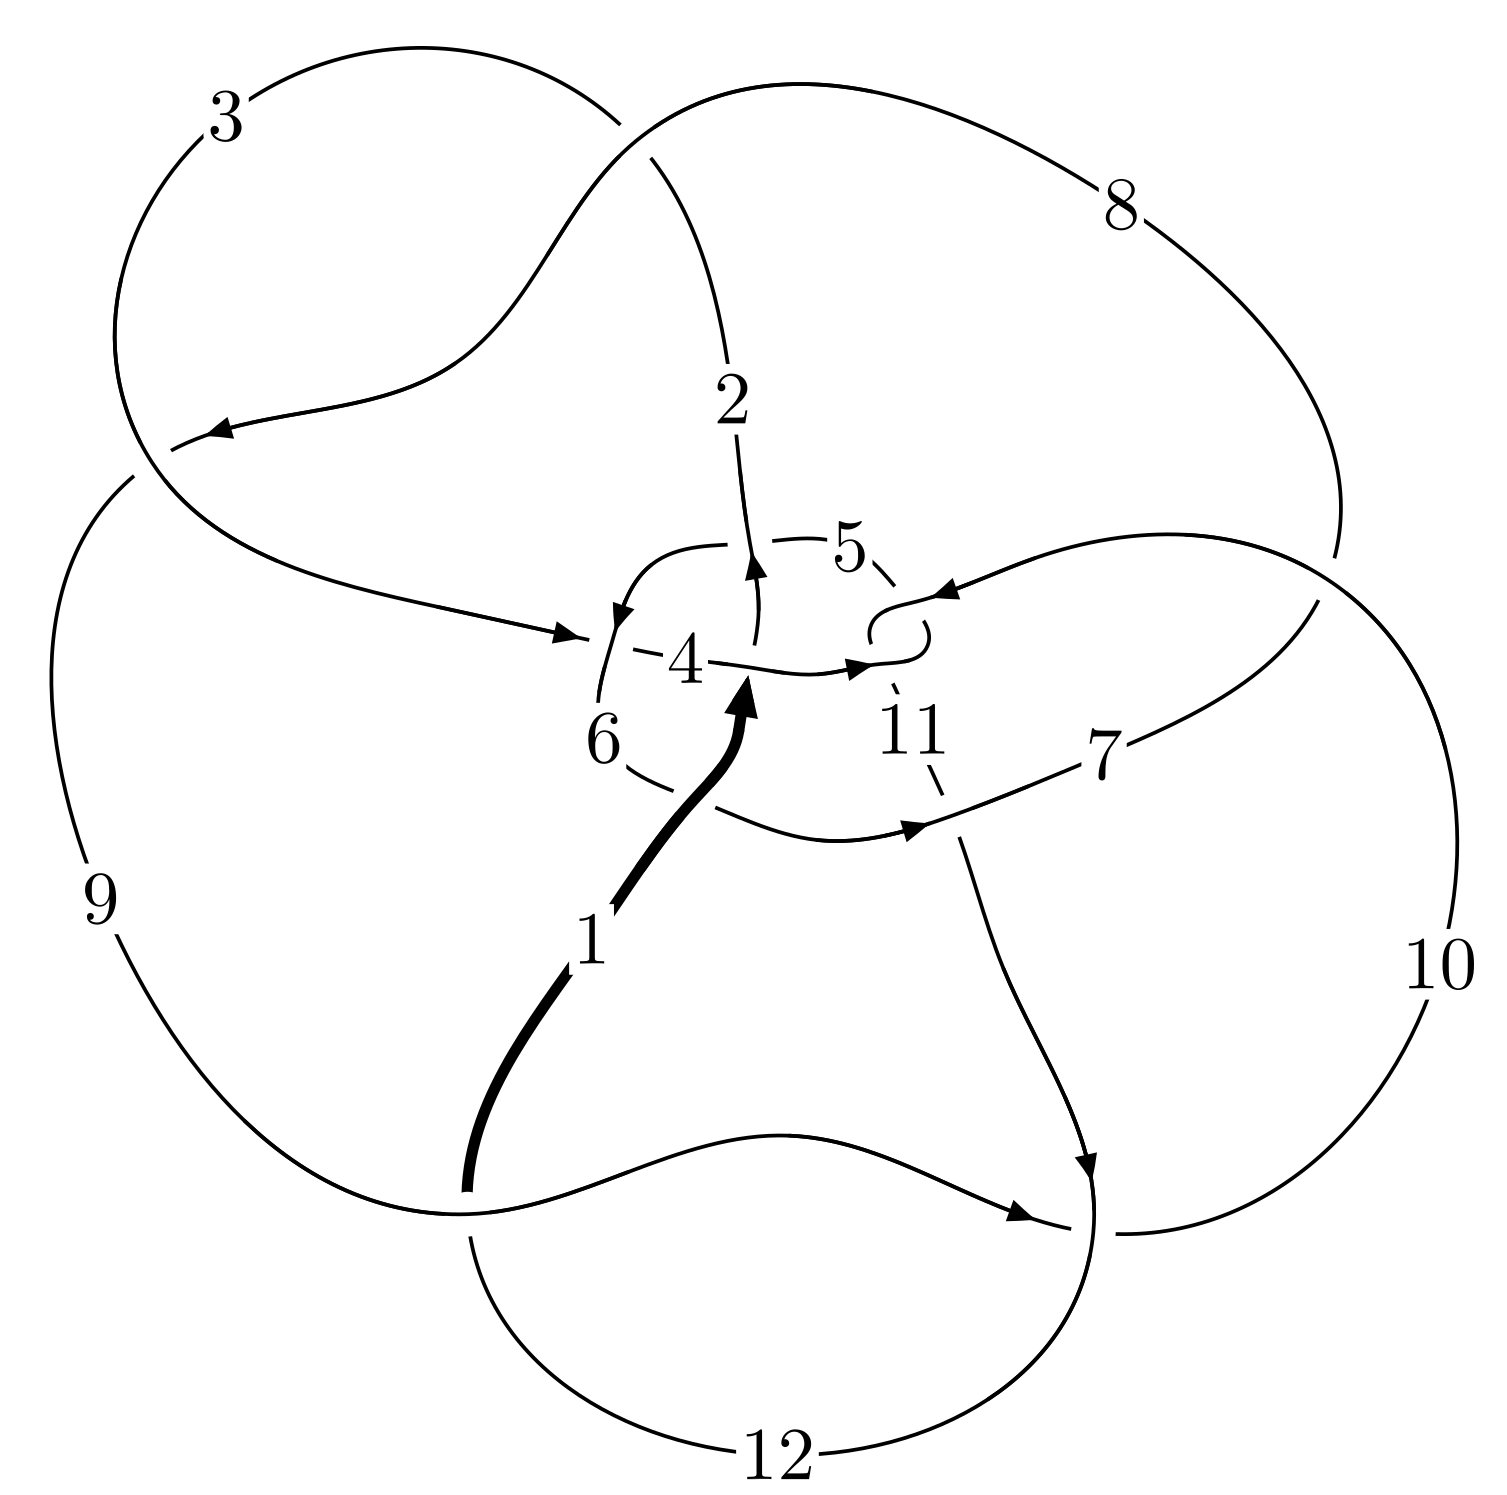
\includegraphics[width=112pt]{../../../GIT/diagram.site/Diagrams/png/2961_12n_0872.png}\\
\ \ \ A knot diagram\footnotemark}&
\allowdisplaybreaks
\textbf{Linearized knot diagam} \\
\cline{2-2}
 &
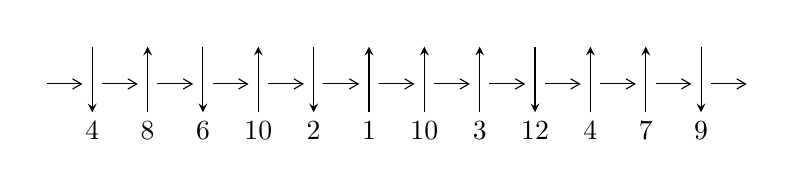
\begin{tikzpicture}[x=20pt, y=17pt]
	% nodes
	\node (C0) at (0, 0) {};
	\node (C1) at (1, 0) {};
	\node (C1U) at (1, +1) {};
	\node (C1D) at (1, -1) {4};

	\node (C2) at (2, 0) {};
	\node (C2U) at (2, +1) {};
	\node (C2D) at (2, -1) {8};

	\node (C3) at (3, 0) {};
	\node (C3U) at (3, +1) {};
	\node (C3D) at (3, -1) {6};

	\node (C4) at (4, 0) {};
	\node (C4U) at (4, +1) {};
	\node (C4D) at (4, -1) {10};

	\node (C5) at (5, 0) {};
	\node (C5U) at (5, +1) {};
	\node (C5D) at (5, -1) {2};

	\node (C6) at (6, 0) {};
	\node (C6U) at (6, +1) {};
	\node (C6D) at (6, -1) {1};

	\node (C7) at (7, 0) {};
	\node (C7U) at (7, +1) {};
	\node (C7D) at (7, -1) {10};

	\node (C8) at (8, 0) {};
	\node (C8U) at (8, +1) {};
	\node (C8D) at (8, -1) {3};

	\node (C9) at (9, 0) {};
	\node (C9U) at (9, +1) {};
	\node (C9D) at (9, -1) {12};

	\node (C10) at (10, 0) {};
	\node (C10U) at (10, +1) {};
	\node (C10D) at (10, -1) {4};

	\node (C11) at (11, 0) {};
	\node (C11U) at (11, +1) {};
	\node (C11D) at (11, -1) {7};

	\node (C12) at (12, 0) {};
	\node (C12U) at (12, +1) {};
	\node (C12D) at (12, -1) {9};
	\node (C13) at (13, 0) {};

	% arrows
	\draw[->,>={angle 60}]
	(C0) edge (C1) (C1) edge (C2) (C2) edge (C3) (C3) edge (C4) (C4) edge (C5) (C5) edge (C6) (C6) edge (C7) (C7) edge (C8) (C8) edge (C9) (C9) edge (C10) (C10) edge (C11) (C11) edge (C12) (C12) edge (C13) ;	\draw[->,>=stealth]
	(C1U) edge (C1D) (C2D) edge (C2U) (C3U) edge (C3D) (C4D) edge (C4U) (C5U) edge (C5D) (C6D) edge (C6U) (C7D) edge (C7U) (C8D) edge (C8U) (C9U) edge (C9D) (C10D) edge (C10U) (C11D) edge (C11U) (C12U) edge (C12D) ;
	\end{tikzpicture} \\
\hhline{~~} \\& 
\textbf{Solving Sequence} \\ \cline{2-2} 
 &
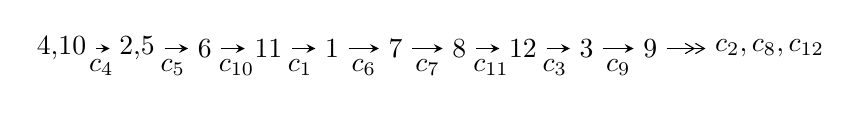
\begin{tikzpicture}[x=23pt, y=7pt]
	% node
	\node (A0) at (-1/8, 0) {4,10};
	\node (A1) at (17/16, 0) {2,5};
	\node (A2) at (17/8, 0) {6};
	\node (A3) at (25/8, 0) {11};
	\node (A4) at (33/8, 0) {1};
	\node (A5) at (41/8, 0) {7};
	\node (A6) at (49/8, 0) {8};
	\node (A7) at (57/8, 0) {12};
	\node (A8) at (65/8, 0) {3};
	\node (A9) at (73/8, 0) {9};
	\node (C1) at (1/2, -1) {$c_{4}$};
	\node (C2) at (13/8, -1) {$c_{5}$};
	\node (C3) at (21/8, -1) {$c_{10}$};
	\node (C4) at (29/8, -1) {$c_{1}$};
	\node (C5) at (37/8, -1) {$c_{6}$};
	\node (C6) at (45/8, -1) {$c_{7}$};
	\node (C7) at (53/8, -1) {$c_{11}$};
	\node (C8) at (61/8, -1) {$c_{3}$};
	\node (C9) at (69/8, -1) {$c_{9}$};
	\node (A10) at (11, 0) {$c_{2},c_{8},c_{12}$};

	% edge
	\draw[->,>=stealth]	
	(A0) edge (A1) (A1) edge (A2) (A2) edge (A3) (A3) edge (A4) (A4) edge (A5) (A5) edge (A6) (A6) edge (A7) (A7) edge (A8) (A8) edge (A9) ;
	\draw[->>,>={angle 60}]	
	(A9) edge (A10);
\end{tikzpicture} \\ 

\end{tabular} \\

\footnotetext{
The image of knot diagram is generated by the software ``\textbf{Draw programme}" developed by Andrew Bartholomew(\url{http://www.layer8.co.uk/maths/draw/index.htm\#Running-draw}), where we modified some parts for our purpose(\url{https://github.com/CATsTAILs/LinksPainter}).
}\phantom \\ \newline 
\centering \textbf{Ideals for irreducible components\footnotemark of $X_{\text{par}}$} 
 
\begin{align*}
I^u_{1}&=\langle 
-9.23788\times10^{617} u^{103}-2.13157\times10^{617} u^{102}+\cdots+4.60669\times10^{619} b-1.99228\times10^{621},\\
\phantom{I^u_{1}}&\phantom{= \langle  }1.16323\times10^{621} u^{103}+2.66509\times10^{620} u^{102}+\cdots+2.21582\times10^{622} a+2.45180\times10^{624},\\
\phantom{I^u_{1}}&\phantom{= \langle  }u^{104}-46 u^{102}+\cdots+1213 u-481\rangle \\
I^u_{2}&=\langle 
3.57205\times10^{41} u^{38}-1.99879\times10^{42} u^{37}+\cdots+2.14995\times10^{42} b+5.04738\times10^{42},\\
\phantom{I^u_{2}}&\phantom{= \langle  }-1.71684\times10^{43} u^{38}+1.96289\times10^{43} u^{37}+\cdots+2.14995\times10^{42} a-6.45705\times10^{43},\;u^{39}- u^{38}+\cdots+6 u+1\rangle \\
\\
\end{align*}
\raggedright * 2 irreducible components of $\dim_{\mathbb{C}}=0$, with total 143 representations.\\
\footnotetext{All coefficients of polynomials are rational numbers. But the coefficients are sometimes approximated in decimal forms when there is not enough margin.}
\newpage
\renewcommand{\arraystretch}{1}
\centering \section*{I. $I^u_{1}= \langle -9.24\times10^{617} u^{103}-2.13\times10^{617} u^{102}+\cdots+4.61\times10^{619} b-1.99\times10^{621},\;1.16\times10^{621} u^{103}+2.67\times10^{620} u^{102}+\cdots+2.22\times10^{622} a+2.45\times10^{624},\;u^{104}-46 u^{102}+\cdots+1213 u-481 \rangle$}
\flushleft \textbf{(i) Arc colorings}\\
\begin{tabular}{m{7pt} m{180pt} m{7pt} m{180pt} }
\flushright $a_{4}=$&$\begin{pmatrix}1\\0\end{pmatrix}$ \\
\flushright $a_{10}=$&$\begin{pmatrix}0\\u\end{pmatrix}$ \\
\flushright $a_{2}=$&$\begin{pmatrix}-0.0524965 u^{103}-0.0120276 u^{102}+\cdots-186.829 u-110.650\\0.0200532 u^{103}+0.00462711 u^{102}+\cdots+74.8146 u+43.2475\end{pmatrix}$ \\
\flushright $a_{5}=$&$\begin{pmatrix}1\\- u^2\end{pmatrix}$ \\
\flushright $a_{6}=$&$\begin{pmatrix}-0.0381236 u^{103}-0.00827763 u^{102}+\cdots-138.937 u-72.1056\\0.0437309 u^{103}+0.0101189 u^{102}+\cdots+163.774 u+92.2742\end{pmatrix}$ \\
\flushright $a_{11}=$&$\begin{pmatrix}u\\u\end{pmatrix}$ \\
\flushright $a_{1}=$&$\begin{pmatrix}-0.0324433 u^{103}-0.00740048 u^{102}+\cdots-112.015 u-67.4025\\0.0200532 u^{103}+0.00462711 u^{102}+\cdots+74.8146 u+43.2475\end{pmatrix}$ \\
\flushright $a_{7}=$&$\begin{pmatrix}0.134160 u^{103}+0.0308828 u^{102}+\cdots+503.351 u+280.897\\0.0829877 u^{103}+0.0195287 u^{102}+\cdots+307.232 u+172.162\end{pmatrix}$ \\
\flushright $a_{8}=$&$\begin{pmatrix}0.134160 u^{103}+0.0308828 u^{102}+\cdots+503.351 u+280.897\\0.0757825 u^{103}+0.0178965 u^{102}+\cdots+280.162 u+157.307\end{pmatrix}$ \\
\flushright $a_{12}=$&$\begin{pmatrix}0.150051 u^{103}+0.0345510 u^{102}+\cdots+576.541 u+307.325\\0.0617242 u^{103}+0.0144059 u^{102}+\cdots+222.546 u+125.979\end{pmatrix}$ \\
\flushright $a_{3}=$&$\begin{pmatrix}-0.128848 u^{103}-0.0292433 u^{102}+\cdots-481.056 u-271.980\\-0.0856454 u^{103}-0.0201046 u^{102}+\cdots-318.073 u-177.623\end{pmatrix}$ \\
\flushright $a_{9}=$&$\begin{pmatrix}0.0927804 u^{103}+0.0225380 u^{102}+\cdots+335.410 u+191.496\\-0.0320252 u^{103}-0.00726549 u^{102}+\cdots-122.725 u-67.7945\end{pmatrix}$\\&\end{tabular}
\flushleft \textbf{(ii) Obstruction class $= -1$}\\~\\
\flushleft \textbf{(iii) Cusp Shapes $= 0.0640073 u^{103}+0.0156871 u^{102}+\cdots+282.714 u+148.258$}\\~\\
\newpage\renewcommand{\arraystretch}{1}
\flushleft \textbf{(iv) u-Polynomials at the component}\newline \\
\begin{tabular}{m{50pt}|m{274pt}}
Crossings & \hspace{64pt}u-Polynomials at each crossing \\
\hline $$\begin{aligned}c_{1}\end{aligned}$$&$\begin{aligned}
&u^{104}-12 u^{103}+\cdots-248936 u-16709
\end{aligned}$\\
\hline $$\begin{aligned}c_{2},c_{8}\end{aligned}$$&$\begin{aligned}
&u^{104}+3 u^{103}+\cdots+113528 u+9059
\end{aligned}$\\
\hline $$\begin{aligned}c_{3}\end{aligned}$$&$\begin{aligned}
&u^{104}-7 u^{103}+\cdots-6 u+1
\end{aligned}$\\
\hline $$\begin{aligned}c_{4},c_{10}\end{aligned}$$&$\begin{aligned}
&u^{104}-46 u^{102}+\cdots-1213 u-481
\end{aligned}$\\
\hline $$\begin{aligned}c_{5}\end{aligned}$$&$\begin{aligned}
&u^{104}+17 u^{102}+\cdots-422700176 u-225656489
\end{aligned}$\\
\hline $$\begin{aligned}c_{6}\end{aligned}$$&$\begin{aligned}
&u^{104}+4 u^{103}+\cdots-39794 u-3223
\end{aligned}$\\
\hline $$\begin{aligned}c_{7}\end{aligned}$$&$\begin{aligned}
&u^{104}+4 u^{103}+\cdots-7017838 u-1565497
\end{aligned}$\\
\hline $$\begin{aligned}c_{9},c_{12}\end{aligned}$$&$\begin{aligned}
&u^{104}-6 u^{103}+\cdots-580 u+71
\end{aligned}$\\
\hline $$\begin{aligned}c_{11}\end{aligned}$$&$\begin{aligned}
&u^{104}-2 u^{103}+\cdots-63017876 u-39654871
\end{aligned}$\\
\hline
\end{tabular}\\~\\
\newpage\renewcommand{\arraystretch}{1}
\flushleft \textbf{(v) Riley Polynomials at the component}\newline \\
\begin{tabular}{m{50pt}|m{274pt}}
Crossings & \hspace{64pt}Riley Polynomials at each crossing \\
\hline $$\begin{aligned}c_{1}\end{aligned}$$&$\begin{aligned}
&y^{104}+46 y^{103}+\cdots-6027901366 y+279190681
\end{aligned}$\\
\hline $$\begin{aligned}c_{2},c_{8}\end{aligned}$$&$\begin{aligned}
&y^{104}-83 y^{103}+\cdots-2711816774 y+82065481
\end{aligned}$\\
\hline $$\begin{aligned}c_{3}\end{aligned}$$&$\begin{aligned}
&y^{104}-21 y^{103}+\cdots-186 y+1
\end{aligned}$\\
\hline $$\begin{aligned}c_{4},c_{10}\end{aligned}$$&$\begin{aligned}
&y^{104}-92 y^{103}+\cdots-6263091 y+231361
\end{aligned}$\\
\hline $$\begin{aligned}c_{5}\end{aligned}$$&$\begin{aligned}
&y^{104}+34 y^{103}+\cdots+567548679396571134 y+50920851027807121
\end{aligned}$\\
\hline $$\begin{aligned}c_{6}\end{aligned}$$&$\begin{aligned}
&y^{104}-32 y^{103}+\cdots+738170736 y+10387729
\end{aligned}$\\
\hline $$\begin{aligned}c_{7}\end{aligned}$$&$\begin{aligned}
&y^{104}-46 y^{103}+\cdots-93370286202562 y+2450780857009
\end{aligned}$\\
\hline $$\begin{aligned}c_{9},c_{12}\end{aligned}$$&$\begin{aligned}
&y^{104}+64 y^{103}+\cdots+348466 y+5041
\end{aligned}$\\
\hline $$\begin{aligned}c_{11}\end{aligned}$$&$\begin{aligned}
&y^{104}-38 y^{103}+\cdots-12842525972544346 y+1572508794026641
\end{aligned}$\\
\hline
\end{tabular}\\~\\
\newpage\flushleft \textbf{(vi) Complex Volumes and Cusp Shapes}
$$\begin{array}{c|c|c}  
\text{Solutions to }I^u_{1}& \I (\text{vol} + \sqrt{-1}CS) & \text{Cusp shape}\\
 \hline 
\begin{aligned}
u &= -0.756388 + 0.614504 I \\
a &= \phantom{-}0.953008 - 0.229351 I \\
b &= -0.239639 + 0.440382 I\end{aligned}
 & \phantom{-}0.84585 - 1.85988 I & \phantom{-0.000000 } 0 \\ \hline\begin{aligned}
u &= -0.756388 - 0.614504 I \\
a &= \phantom{-}0.953008 + 0.229351 I \\
b &= -0.239639 - 0.440382 I\end{aligned}
 & \phantom{-}0.84585 + 1.85988 I & \phantom{-0.000000 } 0 \\ \hline\begin{aligned}
u &= \phantom{-}0.043265 + 1.026080 I \\
a &= \phantom{-}0.046814 + 0.470367 I \\
b &= -0.468872 + 0.940055 I\end{aligned}
 & \phantom{-}1.10399 + 5.81000 I & \phantom{-0.000000 } 0 \\ \hline\begin{aligned}
u &= \phantom{-}0.043265 - 1.026080 I \\
a &= \phantom{-}0.046814 - 0.470367 I \\
b &= -0.468872 - 0.940055 I\end{aligned}
 & \phantom{-}1.10399 - 5.81000 I & \phantom{-0.000000 } 0 \\ \hline\begin{aligned}
u &= \phantom{-}0.559475 + 0.780068 I \\
a &= -1.146960 + 0.561597 I \\
b &= -0.303316 + 0.521127 I\end{aligned}
 & \phantom{-}1.77195 + 6.26844 I & \phantom{-0.000000 } 0 \\ \hline\begin{aligned}
u &= \phantom{-}0.559475 - 0.780068 I \\
a &= -1.146960 - 0.561597 I \\
b &= -0.303316 - 0.521127 I\end{aligned}
 & \phantom{-}1.77195 - 6.26844 I & \phantom{-0.000000 } 0 \\ \hline\begin{aligned}
u &= \phantom{-}0.479752 + 0.972353 I \\
a &= -1.91141 - 1.44571 I \\
b &= -1.028730 + 0.471775 I\end{aligned}
 & -2.99427 + 3.87327 I & \phantom{-0.000000 } 0 \\ \hline\begin{aligned}
u &= \phantom{-}0.479752 - 0.972353 I \\
a &= -1.91141 + 1.44571 I \\
b &= -1.028730 - 0.471775 I\end{aligned}
 & -2.99427 - 3.87327 I & \phantom{-0.000000 } 0 \\ \hline\begin{aligned}
u &= -1.11214\phantom{ +0.000000I} \\
a &= \phantom{-}0.978552\phantom{ +0.000000I} \\
b &= \phantom{-}0.687155\phantom{ +0.000000I}\end{aligned}
 & \phantom{-}1.70571\phantom{ +0.000000I} & \phantom{-0.000000 } 0 \\ \hline\begin{aligned}
u &= \phantom{-}0.257608 + 0.797734 I \\
a &= \phantom{-}0.519153 - 0.274406 I \\
b &= -0.681323 - 0.687497 I\end{aligned}
 & -1.82356 - 1.36255 I & \phantom{-0.000000 } 0\\
 \hline 
 \end{array}$$\newpage$$\begin{array}{c|c|c}  
\text{Solutions to }I^u_{1}& \I (\text{vol} + \sqrt{-1}CS) & \text{Cusp shape}\\
 \hline 
\begin{aligned}
u &= \phantom{-}0.257608 - 0.797734 I \\
a &= \phantom{-}0.519153 + 0.274406 I \\
b &= -0.681323 + 0.687497 I\end{aligned}
 & -1.82356 + 1.36255 I & \phantom{-0.000000 } 0 \\ \hline\begin{aligned}
u &= -0.079941 + 0.815009 I \\
a &= \phantom{-}0.366854 - 0.910951 I \\
b &= -0.407217 - 0.332853 I\end{aligned}
 & -1.77525 - 1.53905 I & \phantom{-0.000000 } 0 \\ \hline\begin{aligned}
u &= -0.079941 - 0.815009 I \\
a &= \phantom{-}0.366854 + 0.910951 I \\
b &= -0.407217 + 0.332853 I\end{aligned}
 & -1.77525 + 1.53905 I & \phantom{-0.000000 } 0 \\ \hline\begin{aligned}
u &= -0.552200 + 1.118290 I \\
a &= \phantom{-}1.52956 - 0.88253 I \\
b &= \phantom{-}1.69002 + 0.24137 I\end{aligned}
 & -0.45824 - 4.15337 I & \phantom{-0.000000 } 0 \\ \hline\begin{aligned}
u &= -0.552200 - 1.118290 I \\
a &= \phantom{-}1.52956 + 0.88253 I \\
b &= \phantom{-}1.69002 - 0.24137 I\end{aligned}
 & -0.45824 + 4.15337 I & \phantom{-0.000000 } 0 \\ \hline\begin{aligned}
u &= -1.237520 + 0.208871 I \\
a &= \phantom{-}0.42277 + 1.36469 I \\
b &= -0.283995 - 1.243000 I\end{aligned}
 & \phantom{-}4.04848 - 3.85454 I & \phantom{-0.000000 } 0 \\ \hline\begin{aligned}
u &= -1.237520 - 0.208871 I \\
a &= \phantom{-}0.42277 - 1.36469 I \\
b &= -0.283995 + 1.243000 I\end{aligned}
 & \phantom{-}4.04848 + 3.85454 I & \phantom{-0.000000 } 0 \\ \hline\begin{aligned}
u &= \phantom{-}1.241120 + 0.205283 I \\
a &= \phantom{-}0.339401 - 1.191240 I \\
b &= -0.278663 + 1.316540 I\end{aligned}
 & \phantom{-}3.18290 + 3.60441 I & \phantom{-0.000000 } 0 \\ \hline\begin{aligned}
u &= \phantom{-}1.241120 - 0.205283 I \\
a &= \phantom{-}0.339401 + 1.191240 I \\
b &= -0.278663 - 1.316540 I\end{aligned}
 & \phantom{-}3.18290 - 3.60441 I & \phantom{-0.000000 } 0 \\ \hline\begin{aligned}
u &= -0.052331 + 1.292450 I \\
a &= -0.0316547 - 0.0907787 I \\
b &= -0.592848 - 0.101762 I\end{aligned}
 & -3.95483 - 1.93894 I & \phantom{-0.000000 } 0\\
 \hline 
 \end{array}$$\newpage$$\begin{array}{c|c|c}  
\text{Solutions to }I^u_{1}& \I (\text{vol} + \sqrt{-1}CS) & \text{Cusp shape}\\
 \hline 
\begin{aligned}
u &= -0.052331 - 1.292450 I \\
a &= -0.0316547 + 0.0907787 I \\
b &= -0.592848 + 0.101762 I\end{aligned}
 & -3.95483 + 1.93894 I & \phantom{-0.000000 } 0 \\ \hline\begin{aligned}
u &= \phantom{-}1.316300 + 0.242283 I \\
a &= \phantom{-}0.699095 + 0.836061 I \\
b &= \phantom{-}0.701758 - 0.503985 I\end{aligned}
 & \phantom{-}5.01156 + 5.64140 I & \phantom{-0.000000 } 0 \\ \hline\begin{aligned}
u &= \phantom{-}1.316300 - 0.242283 I \\
a &= \phantom{-}0.699095 - 0.836061 I \\
b &= \phantom{-}0.701758 + 0.503985 I\end{aligned}
 & \phantom{-}5.01156 - 5.64140 I & \phantom{-0.000000 } 0 \\ \hline\begin{aligned}
u &= -0.174763 + 1.327980 I \\
a &= \phantom{-}0.121819 - 0.136944 I \\
b &= \phantom{-}0.520470 + 1.048980 I\end{aligned}
 & \phantom{-}8.07740 + 0.96350 I & \phantom{-0.000000 } 0 \\ \hline\begin{aligned}
u &= -0.174763 - 1.327980 I \\
a &= \phantom{-}0.121819 + 0.136944 I \\
b &= \phantom{-}0.520470 - 1.048980 I\end{aligned}
 & \phantom{-}8.07740 - 0.96350 I & \phantom{-0.000000 } 0 \\ \hline\begin{aligned}
u &= -0.520435 + 0.354656 I \\
a &= \phantom{-}1.056080 + 0.327009 I \\
b &= -0.450370 - 0.117474 I\end{aligned}
 & \phantom{-}0.84359 - 1.70694 I & \phantom{-}4.49768 + 5.15421 I \\ \hline\begin{aligned}
u &= -0.520435 - 0.354656 I \\
a &= \phantom{-}1.056080 - 0.327009 I \\
b &= -0.450370 + 0.117474 I\end{aligned}
 & \phantom{-}0.84359 + 1.70694 I & \phantom{-}4.49768 - 5.15421 I \\ \hline\begin{aligned}
u &= \phantom{-}0.596675 + 0.201234 I \\
a &= \phantom{-}0.408682 + 0.394693 I \\
b &= \phantom{-}0.238546 - 0.794451 I\end{aligned}
 & \phantom{-}3.32423 - 2.67744 I & \phantom{-}6.96385 + 1.14988 I \\ \hline\begin{aligned}
u &= \phantom{-}0.596675 - 0.201234 I \\
a &= \phantom{-}0.408682 - 0.394693 I \\
b &= \phantom{-}0.238546 + 0.794451 I\end{aligned}
 & \phantom{-}3.32423 + 2.67744 I & \phantom{-}6.96385 - 1.14988 I \\ \hline\begin{aligned}
u &= -1.381170 + 0.256326 I \\
a &= \phantom{-}0.455512 - 0.994438 I \\
b &= \phantom{-}0.173705 + 0.785758 I\end{aligned}
 & \phantom{-}3.20991 - 0.82993 I & \phantom{-0.000000 } 0\\
 \hline 
 \end{array}$$\newpage$$\begin{array}{c|c|c}  
\text{Solutions to }I^u_{1}& \I (\text{vol} + \sqrt{-1}CS) & \text{Cusp shape}\\
 \hline 
\begin{aligned}
u &= -1.381170 - 0.256326 I \\
a &= \phantom{-}0.455512 + 0.994438 I \\
b &= \phantom{-}0.173705 - 0.785758 I\end{aligned}
 & \phantom{-}3.20991 + 0.82993 I & \phantom{-0.000000 } 0 \\ \hline\begin{aligned}
u &= \phantom{-}0.473373 + 0.304198 I \\
a &= \phantom{-}0.780415 + 0.227803 I \\
b &= -1.065160 - 0.452018 I\end{aligned}
 & -1.88690 - 1.07563 I & -0.370812 - 1.040121 I \\ \hline\begin{aligned}
u &= \phantom{-}0.473373 - 0.304198 I \\
a &= \phantom{-}0.780415 - 0.227803 I \\
b &= -1.065160 + 0.452018 I\end{aligned}
 & -1.88690 + 1.07563 I & -0.370812 + 1.040121 I \\ \hline\begin{aligned}
u &= -0.499233 + 0.255636 I \\
a &= \phantom{-}0.498852 + 0.083658 I \\
b &= \phantom{-}0.530811 - 0.422327 I\end{aligned}
 & \phantom{-}1.340360 - 0.220514 I & \phantom{-}8.29449 + 0.78751 I \\ \hline\begin{aligned}
u &= -0.499233 - 0.255636 I \\
a &= \phantom{-}0.498852 - 0.083658 I \\
b &= \phantom{-}0.530811 + 0.422327 I\end{aligned}
 & \phantom{-}1.340360 + 0.220514 I & \phantom{-}8.29449 - 0.78751 I \\ \hline\begin{aligned}
u &= \phantom{-}1.43614 + 0.11613 I \\
a &= \phantom{-}0.383333 + 1.117580 I \\
b &= \phantom{-}0.216582 - 1.063790 I\end{aligned}
 & \phantom{-}7.23064 - 2.27781 I & \phantom{-0.000000 } 0 \\ \hline\begin{aligned}
u &= \phantom{-}1.43614 - 0.11613 I \\
a &= \phantom{-}0.383333 - 1.117580 I \\
b &= \phantom{-}0.216582 + 1.063790 I\end{aligned}
 & \phantom{-}7.23064 + 2.27781 I & \phantom{-0.000000 } 0 \\ \hline\begin{aligned}
u &= -1.43874 + 0.08514 I \\
a &= -0.18808 + 1.43903 I \\
b &= \phantom{-}0.268252 - 1.200850 I\end{aligned}
 & \phantom{-}9.50641 - 2.53195 I & \phantom{-0.000000 } 0 \\ \hline\begin{aligned}
u &= -1.43874 - 0.08514 I \\
a &= -0.18808 - 1.43903 I \\
b &= \phantom{-}0.268252 + 1.200850 I\end{aligned}
 & \phantom{-}9.50641 + 2.53195 I & \phantom{-0.000000 } 0 \\ \hline\begin{aligned}
u &= \phantom{-}0.337037 + 0.433784 I \\
a &= \phantom{-}1.232520 - 0.335320 I \\
b &= -0.983901 + 0.278226 I\end{aligned}
 & -0.53776 + 1.39330 I & \phantom{-}1.75716 + 0.61906 I\\
 \hline 
 \end{array}$$\newpage$$\begin{array}{c|c|c}  
\text{Solutions to }I^u_{1}& \I (\text{vol} + \sqrt{-1}CS) & \text{Cusp shape}\\
 \hline 
\begin{aligned}
u &= \phantom{-}0.337037 - 0.433784 I \\
a &= \phantom{-}1.232520 + 0.335320 I \\
b &= -0.983901 - 0.278226 I\end{aligned}
 & -0.53776 - 1.39330 I & \phantom{-}1.75716 - 0.61906 I \\ \hline\begin{aligned}
u &= -1.45495 + 0.02322 I \\
a &= -0.60993 - 1.34266 I \\
b &= -0.143920 + 0.848854 I\end{aligned}
 & \phantom{-}10.85450 - 6.48839 I & \phantom{-0.000000 } 0 \\ \hline\begin{aligned}
u &= -1.45495 - 0.02322 I \\
a &= -0.60993 + 1.34266 I \\
b &= -0.143920 - 0.848854 I\end{aligned}
 & \phantom{-}10.85450 + 6.48839 I & \phantom{-0.000000 } 0 \\ \hline\begin{aligned}
u &= -0.090629 + 0.518992 I \\
a &= \phantom{-}1.290290 + 0.113821 I \\
b &= -0.992919 - 0.177822 I\end{aligned}
 & -0.848158 - 0.616971 I & \phantom{-}5.30485 + 0.57557 I \\ \hline\begin{aligned}
u &= -0.090629 - 0.518992 I \\
a &= \phantom{-}1.290290 - 0.113821 I \\
b &= -0.992919 + 0.177822 I\end{aligned}
 & -0.848158 + 0.616971 I & \phantom{-}5.30485 - 0.57557 I \\ \hline\begin{aligned}
u &= -0.025369 + 0.510521 I \\
a &= \phantom{-}1.04170 + 2.27833 I \\
b &= -0.109941 + 1.010940 I\end{aligned}
 & \phantom{-}0.96411 - 2.80779 I & \phantom{-}3.93129 - 3.03588 I \\ \hline\begin{aligned}
u &= -0.025369 - 0.510521 I \\
a &= \phantom{-}1.04170 - 2.27833 I \\
b &= -0.109941 - 1.010940 I\end{aligned}
 & \phantom{-}0.96411 + 2.80779 I & \phantom{-}3.93129 + 3.03588 I \\ \hline\begin{aligned}
u &= \phantom{-}0.061045 + 0.493659 I \\
a &= \phantom{-}2.37160 - 0.15194 I \\
b &= \phantom{-}0.947452 + 0.263918 I\end{aligned}
 & -0.25369 - 2.78146 I & \phantom{-}2.20642 + 5.49581 I \\ \hline\begin{aligned}
u &= \phantom{-}0.061045 - 0.493659 I \\
a &= \phantom{-}2.37160 + 0.15194 I \\
b &= \phantom{-}0.947452 - 0.263918 I\end{aligned}
 & -0.25369 + 2.78146 I & \phantom{-}2.20642 - 5.49581 I \\ \hline\begin{aligned}
u &= \phantom{-}0.18426 + 1.49536 I \\
a &= \phantom{-}0.325806 - 0.013730 I \\
b &= -0.190423 - 0.077217 I\end{aligned}
 & -1.71906 + 0.61777 I & \phantom{-0.000000 } 0\\
 \hline 
 \end{array}$$\newpage$$\begin{array}{c|c|c}  
\text{Solutions to }I^u_{1}& \I (\text{vol} + \sqrt{-1}CS) & \text{Cusp shape}\\
 \hline 
\begin{aligned}
u &= \phantom{-}0.18426 - 1.49536 I \\
a &= \phantom{-}0.325806 + 0.013730 I \\
b &= -0.190423 + 0.077217 I\end{aligned}
 & -1.71906 - 0.61777 I & \phantom{-0.000000 } 0 \\ \hline\begin{aligned}
u &= \phantom{-}1.51730 + 0.38462 I \\
a &= \phantom{-}0.002624 - 1.264570 I \\
b &= -0.94235 + 1.62193 I\end{aligned}
 & \phantom{-}2.76297 + 6.27366 I & \phantom{-0.000000 } 0 \\ \hline\begin{aligned}
u &= \phantom{-}1.51730 - 0.38462 I \\
a &= \phantom{-}0.002624 + 1.264570 I \\
b &= -0.94235 - 1.62193 I\end{aligned}
 & \phantom{-}2.76297 - 6.27366 I & \phantom{-0.000000 } 0 \\ \hline\begin{aligned}
u &= -1.56574 + 0.12682 I \\
a &= -0.639263 - 0.502518 I \\
b &= -1.081930 + 0.421284 I\end{aligned}
 & \phantom{-}7.69459 + 6.35826 I & \phantom{-0.000000 } 0 \\ \hline\begin{aligned}
u &= -1.56574 - 0.12682 I \\
a &= -0.639263 + 0.502518 I \\
b &= -1.081930 - 0.421284 I\end{aligned}
 & \phantom{-}7.69459 - 6.35826 I & \phantom{-0.000000 } 0 \\ \hline\begin{aligned}
u &= \phantom{-}1.55933 + 0.22492 I \\
a &= \phantom{-}0.155107 + 1.012440 I \\
b &= \phantom{-}0.274584 - 0.670362 I\end{aligned}
 & \phantom{-}5.23399 + 4.89676 I & \phantom{-0.000000 } 0 \\ \hline\begin{aligned}
u &= \phantom{-}1.55933 - 0.22492 I \\
a &= \phantom{-}0.155107 - 1.012440 I \\
b &= \phantom{-}0.274584 + 0.670362 I\end{aligned}
 & \phantom{-}5.23399 - 4.89676 I & \phantom{-0.000000 } 0 \\ \hline\begin{aligned}
u &= -1.55267 + 0.31896 I \\
a &= -0.096842 + 1.391900 I \\
b &= -0.94876 - 2.49473 I\end{aligned}
 & \phantom{-}5.77660 - 1.06575 I & \phantom{-0.000000 } 0 \\ \hline\begin{aligned}
u &= -1.55267 - 0.31896 I \\
a &= -0.096842 - 1.391900 I \\
b &= -0.94876 + 2.49473 I\end{aligned}
 & \phantom{-}5.77660 + 1.06575 I & \phantom{-0.000000 } 0 \\ \hline\begin{aligned}
u &= \phantom{-}1.58254 + 0.13787 I \\
a &= -0.441432 - 0.916190 I \\
b &= \phantom{-}0.191245 + 1.306220 I\end{aligned}
 & \phantom{-}5.73185 - 6.24754 I & \phantom{-0.000000 } 0\\
 \hline 
 \end{array}$$\newpage$$\begin{array}{c|c|c}  
\text{Solutions to }I^u_{1}& \I (\text{vol} + \sqrt{-1}CS) & \text{Cusp shape}\\
 \hline 
\begin{aligned}
u &= \phantom{-}1.58254 - 0.13787 I \\
a &= -0.441432 + 0.916190 I \\
b &= \phantom{-}0.191245 - 1.306220 I\end{aligned}
 & \phantom{-}5.73185 + 6.24754 I & \phantom{-0.000000 } 0 \\ \hline\begin{aligned}
u &= \phantom{-}1.60273 + 0.13079 I \\
a &= -0.077357 - 1.159800 I \\
b &= \phantom{-}0.172948 + 1.329900 I\end{aligned}
 & \phantom{-}8.08362 + 2.71293 I & \phantom{-0.000000 } 0 \\ \hline\begin{aligned}
u &= \phantom{-}1.60273 - 0.13079 I \\
a &= -0.077357 + 1.159800 I \\
b &= \phantom{-}0.172948 - 1.329900 I\end{aligned}
 & \phantom{-}8.08362 - 2.71293 I & \phantom{-0.000000 } 0 \\ \hline\begin{aligned}
u &= \phantom{-}1.60813 + 0.02386 I \\
a &= -0.250032 + 1.049610 I \\
b &= \phantom{-}0.289823 - 0.885399 I\end{aligned}
 & \phantom{-}5.89098 + 4.69416 I & \phantom{-0.000000 } 0 \\ \hline\begin{aligned}
u &= \phantom{-}1.60813 - 0.02386 I \\
a &= -0.250032 - 1.049610 I \\
b &= \phantom{-}0.289823 + 0.885399 I\end{aligned}
 & \phantom{-}5.89098 - 4.69416 I & \phantom{-0.000000 } 0 \\ \hline\begin{aligned}
u &= -1.59173 + 0.37969 I \\
a &= \phantom{-}0.044658 + 1.232300 I \\
b &= -1.10744 - 1.54241 I\end{aligned}
 & \phantom{-}6.91684 - 11.13780 I & \phantom{-0.000000 } 0 \\ \hline\begin{aligned}
u &= -1.59173 - 0.37969 I \\
a &= \phantom{-}0.044658 - 1.232300 I \\
b &= -1.10744 + 1.54241 I\end{aligned}
 & \phantom{-}6.91684 + 11.13780 I & \phantom{-0.000000 } 0 \\ \hline\begin{aligned}
u &= \phantom{-}1.64848 + 0.01689 I \\
a &= -0.395136 - 0.733982 I \\
b &= \phantom{-}2.09514 + 1.15918 I\end{aligned}
 & \phantom{-}9.53284 + 7.96172 I & \phantom{-0.000000 } 0 \\ \hline\begin{aligned}
u &= \phantom{-}1.64848 - 0.01689 I \\
a &= -0.395136 + 0.733982 I \\
b &= \phantom{-}2.09514 - 1.15918 I\end{aligned}
 & \phantom{-}9.53284 - 7.96172 I & \phantom{-0.000000 } 0 \\ \hline\begin{aligned}
u &= -1.64310 + 0.13786 I \\
a &= -0.364892 + 0.902513 I \\
b &= \phantom{-}0.43140 - 1.45698 I\end{aligned}
 & \phantom{-}5.18984 + 2.46675 I & \phantom{-0.000000 } 0\\
 \hline 
 \end{array}$$\newpage$$\begin{array}{c|c|c}  
\text{Solutions to }I^u_{1}& \I (\text{vol} + \sqrt{-1}CS) & \text{Cusp shape}\\
 \hline 
\begin{aligned}
u &= -1.64310 - 0.13786 I \\
a &= -0.364892 - 0.902513 I \\
b &= \phantom{-}0.43140 + 1.45698 I\end{aligned}
 & \phantom{-}5.18984 - 2.46675 I & \phantom{-0.000000 } 0 \\ \hline\begin{aligned}
u &= -0.166413 + 0.298634 I \\
a &= \phantom{-}3.16526 + 1.96290 I \\
b &= \phantom{-}0.828427 - 0.529954 I\end{aligned}
 & \phantom{-}6.21785 + 5.73133 I & \phantom{-}5.01843 - 6.13992 I \\ \hline\begin{aligned}
u &= -0.166413 - 0.298634 I \\
a &= \phantom{-}3.16526 - 1.96290 I \\
b &= \phantom{-}0.828427 + 0.529954 I\end{aligned}
 & \phantom{-}6.21785 - 5.73133 I & \phantom{-}5.01843 + 6.13992 I \\ \hline\begin{aligned}
u &= \phantom{-}1.66740\phantom{ +0.000000I} \\
a &= -0.621700\phantom{ +0.000000I} \\
b &= -1.22807\phantom{ +0.000000I}\end{aligned}
 & \phantom{-}3.12880\phantom{ +0.000000I} & \phantom{-0.000000 } 0 \\ \hline\begin{aligned}
u &= \phantom{-}1.66090 + 0.15762 I \\
a &= -0.414612 - 0.909175 I \\
b &= \phantom{-}1.19545 + 1.41298 I\end{aligned}
 & \phantom{-}12.88540 - 3.37022 I & \phantom{-0.000000 } 0 \\ \hline\begin{aligned}
u &= \phantom{-}1.66090 - 0.15762 I \\
a &= -0.414612 + 0.909175 I \\
b &= \phantom{-}1.19545 - 1.41298 I\end{aligned}
 & \phantom{-}12.88540 + 3.37022 I & \phantom{-0.000000 } 0 \\ \hline\begin{aligned}
u &= \phantom{-}0.323065 + 0.053749 I \\
a &= \phantom{-}6.12307 + 1.87193 I \\
b &= -0.208011 - 0.846828 I\end{aligned}
 & -2.44406 - 2.53576 I & \phantom{-}5.95296 + 7.08262 I \\ \hline\begin{aligned}
u &= \phantom{-}0.323065 - 0.053749 I \\
a &= \phantom{-}6.12307 - 1.87193 I \\
b &= -0.208011 + 0.846828 I\end{aligned}
 & -2.44406 + 2.53576 I & \phantom{-}5.95296 - 7.08262 I \\ \hline\begin{aligned}
u &= -0.10274 + 1.67429 I \\
a &= \phantom{-}0.0921413 + 0.0591271 I \\
b &= \phantom{-}0.56502 - 1.30388 I\end{aligned}
 & \phantom{-}2.51947 + 3.44695 I & \phantom{-0.000000 } 0 \\ \hline\begin{aligned}
u &= -0.10274 - 1.67429 I \\
a &= \phantom{-}0.0921413 - 0.0591271 I \\
b &= \phantom{-}0.56502 + 1.30388 I\end{aligned}
 & \phantom{-}2.51947 - 3.44695 I & \phantom{-0.000000 } 0\\
 \hline 
 \end{array}$$\newpage$$\begin{array}{c|c|c}  
\text{Solutions to }I^u_{1}& \I (\text{vol} + \sqrt{-1}CS) & \text{Cusp shape}\\
 \hline 
\begin{aligned}
u &= \phantom{-}1.54450 + 0.76341 I \\
a &= \phantom{-}0.359265 + 1.206980 I \\
b &= \phantom{-}1.18244 - 1.28426 I\end{aligned}
 & \phantom{-}12.8242 + 6.3084 I & \phantom{-0.000000 } 0 \\ \hline\begin{aligned}
u &= \phantom{-}1.54450 - 0.76341 I \\
a &= \phantom{-}0.359265 - 1.206980 I \\
b &= \phantom{-}1.18244 + 1.28426 I\end{aligned}
 & \phantom{-}12.8242 - 6.3084 I & \phantom{-0.000000 } 0 \\ \hline\begin{aligned}
u &= -1.73970 + 0.05367 I \\
a &= -0.296579 + 0.866963 I \\
b &= \phantom{-}0.609796 - 0.896396 I\end{aligned}
 & \phantom{-}8.21686 + 6.53641 I & \phantom{-0.000000 } 0 \\ \hline\begin{aligned}
u &= -1.73970 - 0.05367 I \\
a &= -0.296579 - 0.866963 I \\
b &= \phantom{-}0.609796 + 0.896396 I\end{aligned}
 & \phantom{-}8.21686 - 6.53641 I & \phantom{-0.000000 } 0 \\ \hline\begin{aligned}
u &= -1.74903 + 0.15975 I \\
a &= -0.664116 + 0.965931 I \\
b &= \phantom{-}2.06036 - 2.62689 I\end{aligned}
 & \phantom{-}6.33606 - 0.80961 I & \phantom{-0.000000 } 0 \\ \hline\begin{aligned}
u &= -1.74903 - 0.15975 I \\
a &= -0.664116 - 0.965931 I \\
b &= \phantom{-}2.06036 + 2.62689 I\end{aligned}
 & \phantom{-}6.33606 + 0.80961 I & \phantom{-0.000000 } 0 \\ \hline\begin{aligned}
u &= \phantom{-}0.232422 + 0.001806 I \\
a &= \phantom{-}1.61246 + 1.60544 I \\
b &= \phantom{-}1.111540 - 0.606422 I\end{aligned}
 & \phantom{-}1.09944 + 7.69062 I & \phantom{-}9.29665 - 1.98480 I \\ \hline\begin{aligned}
u &= \phantom{-}0.232422 - 0.001806 I \\
a &= \phantom{-}1.61246 - 1.60544 I \\
b &= \phantom{-}1.111540 + 0.606422 I\end{aligned}
 & \phantom{-}1.09944 - 7.69062 I & \phantom{-}9.29665 + 1.98480 I \\ \hline\begin{aligned}
u &= -0.184348 + 0.131797 I \\
a &= \phantom{-}7.96561 + 8.61699 I \\
b &= \phantom{-}0.032242 - 0.731472 I\end{aligned}
 & \phantom{-}2.63552 - 8.00089 I & \phantom{-}13.8289 + 5.2451 I \\ \hline\begin{aligned}
u &= -0.184348 - 0.131797 I \\
a &= \phantom{-}7.96561 - 8.61699 I \\
b &= \phantom{-}0.032242 + 0.731472 I\end{aligned}
 & \phantom{-}2.63552 + 8.00089 I & \phantom{-}13.8289 - 5.2451 I\\
 \hline 
 \end{array}$$\newpage$$\begin{array}{c|c|c}  
\text{Solutions to }I^u_{1}& \I (\text{vol} + \sqrt{-1}CS) & \text{Cusp shape}\\
 \hline 
\begin{aligned}
u &= \phantom{-}1.62585 + 0.71969 I \\
a &= -0.341893 - 0.759788 I \\
b &= -0.346088 + 1.177830 I\end{aligned}
 & \phantom{-}8.01378 + 4.66019 I & \phantom{-0.000000 } 0 \\ \hline\begin{aligned}
u &= \phantom{-}1.62585 - 0.71969 I \\
a &= -0.341893 + 0.759788 I \\
b &= -0.346088 - 1.177830 I\end{aligned}
 & \phantom{-}8.01378 - 4.66019 I & \phantom{-0.000000 } 0 \\ \hline\begin{aligned}
u &= -0.096357 + 0.189225 I \\
a &= \phantom{-}1.84010 - 1.28802 I \\
b &= \phantom{-}1.099090 + 0.511799 I\end{aligned}
 & -0.37155 - 4.63756 I & \phantom{-}5.92962 + 12.03433 I \\ \hline\begin{aligned}
u &= -0.096357 - 0.189225 I \\
a &= \phantom{-}1.84010 + 1.28802 I \\
b &= \phantom{-}1.099090 - 0.511799 I\end{aligned}
 & -0.37155 + 4.63756 I & \phantom{-}5.92962 - 12.03433 I \\ \hline\begin{aligned}
u &= -0.08271 + 1.80979 I \\
a &= \phantom{-}0.0552974 - 0.0688722 I \\
b &= \phantom{-}0.364543 + 1.297180 I\end{aligned}
 & \phantom{-}5.71209 - 9.57896 I & \phantom{-0.000000 } 0 \\ \hline\begin{aligned}
u &= -0.08271 - 1.80979 I \\
a &= \phantom{-}0.0552974 + 0.0688722 I \\
b &= \phantom{-}0.364543 - 1.297180 I\end{aligned}
 & \phantom{-}5.71209 + 9.57896 I & \phantom{-0.000000 } 0 \\ \hline\begin{aligned}
u &= -1.64125 + 0.86922 I \\
a &= -0.309707 + 0.660661 I \\
b &= -0.447918 - 1.094930 I\end{aligned}
 & \phantom{-}12.0338 - 9.2583 I & \phantom{-0.000000 } 0 \\ \hline\begin{aligned}
u &= -1.64125 - 0.86922 I \\
a &= -0.309707 - 0.660661 I \\
b &= -0.447918 + 1.094930 I\end{aligned}
 & \phantom{-}12.0338 + 9.2583 I & \phantom{-0.000000 } 0 \\ \hline\begin{aligned}
u &= \phantom{-}1.72596 + 0.69271 I \\
a &= \phantom{-}0.176980 + 1.109110 I \\
b &= \phantom{-}1.09514 - 1.44804 I\end{aligned}
 & \phantom{-}11.5105 + 18.3276 I & \phantom{-0.000000 } 0 \\ \hline\begin{aligned}
u &= \phantom{-}1.72596 - 0.69271 I \\
a &= \phantom{-}0.176980 - 1.109110 I \\
b &= \phantom{-}1.09514 + 1.44804 I\end{aligned}
 & \phantom{-}11.5105 - 18.3276 I & \phantom{-0.000000 } 0\\
 \hline 
 \end{array}$$\newpage$$\begin{array}{c|c|c}  
\text{Solutions to }I^u_{1}& \I (\text{vol} + \sqrt{-1}CS) & \text{Cusp shape}\\
 \hline 
\begin{aligned}
u &= -1.69905 + 0.75774 I \\
a &= \phantom{-}0.250741 - 1.095290 I \\
b &= \phantom{-}1.16105 + 1.43310 I\end{aligned}
 & \phantom{-}7.5758 - 12.1822 I & \phantom{-0.000000 } 0 \\ \hline\begin{aligned}
u &= -1.69905 - 0.75774 I \\
a &= \phantom{-}0.250741 + 1.095290 I \\
b &= \phantom{-}1.16105 - 1.43310 I\end{aligned}
 & \phantom{-}7.5758 + 12.1822 I & \phantom{-0.000000 } 0 \\ \hline\begin{aligned}
u &= -1.81637 + 0.71837 I \\
a &= -0.238109 + 0.780834 I \\
b &= -0.47363 - 1.36093 I\end{aligned}
 & \phantom{-}11.24820 + 0.27627 I & \phantom{-0.000000 } 0 \\ \hline\begin{aligned}
u &= -1.81637 - 0.71837 I \\
a &= -0.238109 - 0.780834 I \\
b &= -0.47363 + 1.36093 I\end{aligned}
 & \phantom{-}11.24820 - 0.27627 I & \phantom{-0.000000 } 0\\
 \hline 
 \end{array}$$\newpage\newpage\renewcommand{\arraystretch}{1}
\centering \section*{II. $I^u_{2}= \langle 3.57\times10^{41} u^{38}-2.00\times10^{42} u^{37}+\cdots+2.15\times10^{42} b+5.05\times10^{42},\;-1.72\times10^{43} u^{38}+1.96\times10^{43} u^{37}+\cdots+2.15\times10^{42} a-6.46\times10^{43},\;u^{39}- u^{38}+\cdots+6 u+1 \rangle$}
\flushleft \textbf{(i) Arc colorings}\\
\begin{tabular}{m{7pt} m{180pt} m{7pt} m{180pt} }
\flushright $a_{4}=$&$\begin{pmatrix}1\\0\end{pmatrix}$ \\
\flushright $a_{10}=$&$\begin{pmatrix}0\\u\end{pmatrix}$ \\
\flushright $a_{2}=$&$\begin{pmatrix}7.98548 u^{38}-9.12995 u^{37}+\cdots+81.0981 u+30.0335\\-0.166146 u^{38}+0.929693 u^{37}+\cdots+1.67110 u-2.34768\end{pmatrix}$ \\
\flushright $a_{5}=$&$\begin{pmatrix}1\\- u^2\end{pmatrix}$ \\
\flushright $a_{6}=$&$\begin{pmatrix}-7.79895 u^{38}+9.46660 u^{37}+\cdots-79.2390 u-29.2786\\1.60711 u^{38}-0.715761 u^{37}+\cdots+17.0296 u+4.72651\end{pmatrix}$ \\
\flushright $a_{11}=$&$\begin{pmatrix}u\\u\end{pmatrix}$ \\
\flushright $a_{1}=$&$\begin{pmatrix}7.81934 u^{38}-8.20026 u^{37}+\cdots+82.7692 u+27.6859\\-0.166146 u^{38}+0.929693 u^{37}+\cdots+1.67110 u-2.34768\end{pmatrix}$ \\
\flushright $a_{7}=$&$\begin{pmatrix}-5.03822 u^{38}+8.07873 u^{37}+\cdots-38.0591 u-19.7559\\3.70352 u^{38}-2.35693 u^{37}+\cdots+40.4455 u+11.0152\end{pmatrix}$ \\
\flushright $a_{8}=$&$\begin{pmatrix}-5.03822 u^{38}+8.07873 u^{37}+\cdots-38.0591 u-19.7559\\3.90266 u^{38}-2.45839 u^{37}+\cdots+53.6503 u+14.0557\end{pmatrix}$ \\
\flushright $a_{12}=$&$\begin{pmatrix}7.59285 u^{38}-9.38603 u^{37}+\cdots+65.4431 u+27.8874\\1.40118 u^{38}-2.14980 u^{37}+\cdots+8.57664 u+3.91192\end{pmatrix}$ \\
\flushright $a_{3}=$&$\begin{pmatrix}6.37281 u^{38}-9.21544 u^{37}+\cdots+60.7681 u+26.4002\\-2.71720 u^{38}+0.940791 u^{37}+\cdots-39.0238 u-9.32125\end{pmatrix}$ \\
\flushright $a_{9}=$&$\begin{pmatrix}-6.44687 u^{38}+7.05539 u^{37}+\cdots-57.6520 u-20.8889\\1.10191 u^{38}-1.92891 u^{37}+\cdots+21.2655 u+8.42309\end{pmatrix}$\\&\end{tabular}
\flushleft \textbf{(ii) Obstruction class $= 1$}\\~\\
\flushleft \textbf{(iii) Cusp Shapes $= 17.4964 u^{38}-17.4105 u^{37}+\cdots+159.113 u+50.7900$}\\~\\
\newpage\renewcommand{\arraystretch}{1}
\flushleft \textbf{(iv) u-Polynomials at the component}\newline \\
\begin{tabular}{m{50pt}|m{274pt}}
Crossings & \hspace{64pt}u-Polynomials at each crossing \\
\hline $$\begin{aligned}c_{1}\end{aligned}$$&$\begin{aligned}
&u^{39}+u^{38}+\cdots+5 u-1
\end{aligned}$\\
\hline $$\begin{aligned}c_{2}\end{aligned}$$&$\begin{aligned}
&u^{39}-2 u^{38}+\cdots+3 u-1
\end{aligned}$\\
\hline $$\begin{aligned}c_{3}\end{aligned}$$&$\begin{aligned}
&u^{39}-12 u^{38}+\cdots+3 u-1
\end{aligned}$\\
\hline $$\begin{aligned}c_{4}\end{aligned}$$&$\begin{aligned}
&u^{39}- u^{38}+\cdots+6 u+1
\end{aligned}$\\
\hline $$\begin{aligned}c_{5}\end{aligned}$$&$\begin{aligned}
&u^{39}+5 u^{38}+\cdots+9 u+1
\end{aligned}$\\
\hline $$\begin{aligned}c_{6}\end{aligned}$$&$\begin{aligned}
&u^{39}- u^{38}+\cdots+u+1
\end{aligned}$\\
\hline $$\begin{aligned}c_{7}\end{aligned}$$&$\begin{aligned}
&u^{39}+9 u^{38}+\cdots-27 u-1
\end{aligned}$\\
\hline $$\begin{aligned}c_{8}\end{aligned}$$&$\begin{aligned}
&u^{39}+2 u^{38}+\cdots+3 u+1
\end{aligned}$\\
\hline $$\begin{aligned}c_{9}\end{aligned}$$&$\begin{aligned}
&u^{39}-7 u^{38}+\cdots-111 u+17
\end{aligned}$\\
\hline $$\begin{aligned}c_{10}\end{aligned}$$&$\begin{aligned}
&u^{39}+u^{38}+\cdots+6 u-1
\end{aligned}$\\
\hline $$\begin{aligned}c_{11}\end{aligned}$$&$\begin{aligned}
&u^{39}+u^{38}+\cdots+u-1
\end{aligned}$\\
\hline $$\begin{aligned}c_{12}\end{aligned}$$&$\begin{aligned}
&u^{39}+7 u^{38}+\cdots-111 u-17
\end{aligned}$\\
\hline
\end{tabular}\\~\\
\newpage\renewcommand{\arraystretch}{1}
\flushleft \textbf{(v) Riley Polynomials at the component}\newline \\
\begin{tabular}{m{50pt}|m{274pt}}
Crossings & \hspace{64pt}Riley Polynomials at each crossing \\
\hline $$\begin{aligned}c_{1}\end{aligned}$$&$\begin{aligned}
&y^{39}+11 y^{38}+\cdots+9 y-1
\end{aligned}$\\
\hline $$\begin{aligned}c_{2},c_{8}\end{aligned}$$&$\begin{aligned}
&y^{39}-30 y^{38}+\cdots+21 y-1
\end{aligned}$\\
\hline $$\begin{aligned}c_{3}\end{aligned}$$&$\begin{aligned}
&y^{39}-24 y^{38}+\cdots-51 y-1
\end{aligned}$\\
\hline $$\begin{aligned}c_{4},c_{10}\end{aligned}$$&$\begin{aligned}
&y^{39}-15 y^{38}+\cdots+10 y-1
\end{aligned}$\\
\hline $$\begin{aligned}c_{5}\end{aligned}$$&$\begin{aligned}
&y^{39}-21 y^{38}+\cdots-419 y-1
\end{aligned}$\\
\hline $$\begin{aligned}c_{6}\end{aligned}$$&$\begin{aligned}
&y^{39}-11 y^{38}+\cdots-69 y-1
\end{aligned}$\\
\hline $$\begin{aligned}c_{7}\end{aligned}$$&$\begin{aligned}
&y^{39}+15 y^{38}+\cdots+117 y-1
\end{aligned}$\\
\hline $$\begin{aligned}c_{9},c_{12}\end{aligned}$$&$\begin{aligned}
&y^{39}+21 y^{38}+\cdots-6243 y-289
\end{aligned}$\\
\hline $$\begin{aligned}c_{11}\end{aligned}$$&$\begin{aligned}
&y^{39}+11 y^{38}+\cdots-23 y-1
\end{aligned}$\\
\hline
\end{tabular}\\~\\
\newpage\flushleft \textbf{(vi) Complex Volumes and Cusp Shapes}
$$\begin{array}{c|c|c}  
\text{Solutions to }I^u_{2}& \I (\text{vol} + \sqrt{-1}CS) & \text{Cusp shape}\\
 \hline 
\begin{aligned}
u &= -0.714234 + 0.646090 I \\
a &= \phantom{-}0.567389 - 0.166197 I \\
b &= -0.897728 + 0.002371 I\end{aligned}
 & -0.42956 - 2.08315 I & \phantom{-}1.07908 + 10.26660 I \\ \hline\begin{aligned}
u &= -0.714234 - 0.646090 I \\
a &= \phantom{-}0.567389 + 0.166197 I \\
b &= -0.897728 - 0.002371 I\end{aligned}
 & -0.42956 + 2.08315 I & \phantom{-}1.07908 - 10.26660 I \\ \hline\begin{aligned}
u &= \phantom{-}0.481158 + 0.998076 I \\
a &= \phantom{-}1.67117 + 1.11651 I \\
b &= \phantom{-}1.66742 + 0.03836 I\end{aligned}
 & -0.68641 + 4.30104 I & -8.2586 - 15.9444 I \\ \hline\begin{aligned}
u &= \phantom{-}0.481158 - 0.998076 I \\
a &= \phantom{-}1.67117 - 1.11651 I \\
b &= \phantom{-}1.66742 - 0.03836 I\end{aligned}
 & -0.68641 - 4.30104 I & -8.2586 + 15.9444 I \\ \hline\begin{aligned}
u &= \phantom{-}1.112590 + 0.017384 I \\
a &= \phantom{-}0.745644 + 1.198550 I \\
b &= -0.113319 - 1.246330 I\end{aligned}
 & \phantom{-}4.15102 - 4.90321 I & \phantom{-}6.96774 + 7.97063 I \\ \hline\begin{aligned}
u &= \phantom{-}1.112590 - 0.017384 I \\
a &= \phantom{-}0.745644 - 1.198550 I \\
b &= -0.113319 + 1.246330 I\end{aligned}
 & \phantom{-}4.15102 + 4.90321 I & \phantom{-}6.96774 - 7.97063 I \\ \hline\begin{aligned}
u &= -0.222731 + 0.835366 I \\
a &= \phantom{-}0.337960 - 0.239393 I \\
b &= -0.799132 + 0.439136 I\end{aligned}
 & -1.73712 + 0.24562 I & -2.41052 + 2.12061 I \\ \hline\begin{aligned}
u &= -0.222731 - 0.835366 I \\
a &= \phantom{-}0.337960 + 0.239393 I \\
b &= -0.799132 - 0.439136 I\end{aligned}
 & -1.73712 - 0.24562 I & -2.41052 - 2.12061 I \\ \hline\begin{aligned}
u &= \phantom{-}0.375900 + 0.690760 I \\
a &= \phantom{-}2.01354 - 0.71595 I \\
b &= \phantom{-}0.303125 - 1.354280 I\end{aligned}
 & \phantom{-}1.12137 + 3.36026 I & \phantom{-}9.5968 - 11.1830 I \\ \hline\begin{aligned}
u &= \phantom{-}0.375900 - 0.690760 I \\
a &= \phantom{-}2.01354 + 0.71595 I \\
b &= \phantom{-}0.303125 + 1.354280 I\end{aligned}
 & \phantom{-}1.12137 - 3.36026 I & \phantom{-}9.5968 + 11.1830 I\\
 \hline 
 \end{array}$$\newpage$$\begin{array}{c|c|c}  
\text{Solutions to }I^u_{2}& \I (\text{vol} + \sqrt{-1}CS) & \text{Cusp shape}\\
 \hline 
\begin{aligned}
u &= -0.454300 + 1.145050 I \\
a &= -1.77685 + 1.04562 I \\
b &= -1.070190 - 0.458548 I\end{aligned}
 & -2.63420 - 3.92959 I & \phantom{-}8.09206 + 6.77888 I \\ \hline\begin{aligned}
u &= -0.454300 - 1.145050 I \\
a &= -1.77685 - 1.04562 I \\
b &= -1.070190 + 0.458548 I\end{aligned}
 & -2.63420 + 3.92959 I & \phantom{-}8.09206 - 6.77888 I \\ \hline\begin{aligned}
u &= -1.24851\phantom{ +0.000000I} \\
a &= -1.17716\phantom{ +0.000000I} \\
b &= -0.780352\phantom{ +0.000000I}\end{aligned}
 & \phantom{-}1.41069\phantom{ +0.000000I} & -14.4990\phantom{ +0.000000I} \\ \hline\begin{aligned}
u &= \phantom{-}1.272260 + 0.166109 I \\
a &= -0.869963 - 0.952108 I \\
b &= -0.693692 + 0.551477 I\end{aligned}
 & \phantom{-}5.03700 + 5.96400 I & \phantom{-}6.7854 - 17.7637 I \\ \hline\begin{aligned}
u &= \phantom{-}1.272260 - 0.166109 I \\
a &= -0.869963 + 0.952108 I \\
b &= -0.693692 - 0.551477 I\end{aligned}
 & \phantom{-}5.03700 - 5.96400 I & \phantom{-}6.7854 + 17.7637 I \\ \hline\begin{aligned}
u &= \phantom{-}0.311211 + 0.596597 I \\
a &= \phantom{-}0.172876 + 0.158815 I \\
b &= \phantom{-}1.111070 + 0.652901 I\end{aligned}
 & -0.57987 - 4.15092 I & \phantom{-}0.15664 - 1.51083 I \\ \hline\begin{aligned}
u &= \phantom{-}0.311211 - 0.596597 I \\
a &= \phantom{-}0.172876 - 0.158815 I \\
b &= \phantom{-}1.111070 - 0.652901 I\end{aligned}
 & -0.57987 + 4.15092 I & \phantom{-}0.15664 + 1.51083 I \\ \hline\begin{aligned}
u &= \phantom{-}0.312657 + 0.572753 I \\
a &= \phantom{-}0.215966 - 0.166208 I \\
b &= \phantom{-}0.990024 - 0.564976 I\end{aligned}
 & \phantom{-}0.68699 + 8.04590 I & -2.39016 - 12.20225 I \\ \hline\begin{aligned}
u &= \phantom{-}0.312657 - 0.572753 I \\
a &= \phantom{-}0.215966 + 0.166208 I \\
b &= \phantom{-}0.990024 + 0.564976 I\end{aligned}
 & \phantom{-}0.68699 - 8.04590 I & -2.39016 + 12.20225 I \\ \hline\begin{aligned}
u &= -0.173412 + 0.621258 I \\
a &= -0.68541 - 3.69947 I \\
b &= -0.053529 - 0.487116 I\end{aligned}
 & \phantom{-}2.21579 - 8.10973 I & -3.82432 + 10.35697 I\\
 \hline 
 \end{array}$$\newpage$$\begin{array}{c|c|c}  
\text{Solutions to }I^u_{2}& \I (\text{vol} + \sqrt{-1}CS) & \text{Cusp shape}\\
 \hline 
\begin{aligned}
u &= -0.173412 - 0.621258 I \\
a &= -0.68541 + 3.69947 I \\
b &= -0.053529 + 0.487116 I\end{aligned}
 & \phantom{-}2.21579 + 8.10973 I & -3.82432 - 10.35697 I \\ \hline\begin{aligned}
u &= \phantom{-}0.128428 + 1.376150 I \\
a &= \phantom{-}0.310283 - 0.006319 I \\
b &= -0.491663 + 0.093070 I\end{aligned}
 & -1.91949 + 0.73835 I & -14.3543 - 11.4356 I \\ \hline\begin{aligned}
u &= \phantom{-}0.128428 - 1.376150 I \\
a &= \phantom{-}0.310283 + 0.006319 I \\
b &= -0.491663 - 0.093070 I\end{aligned}
 & -1.91949 - 0.73835 I & -14.3543 + 11.4356 I \\ \hline\begin{aligned}
u &= -1.369690 + 0.203673 I \\
a &= \phantom{-}0.279040 + 1.137730 I \\
b &= -0.32764 - 1.39829 I\end{aligned}
 & \phantom{-}2.77371 - 3.09104 I & \phantom{-0.000000 } 0 \\ \hline\begin{aligned}
u &= -1.369690 - 0.203673 I \\
a &= \phantom{-}0.279040 - 1.137730 I \\
b &= -0.32764 + 1.39829 I\end{aligned}
 & \phantom{-}2.77371 + 3.09104 I & \phantom{-0.000000 } 0 \\ \hline\begin{aligned}
u &= -1.40802 + 0.13736 I \\
a &= -0.604487 + 1.106370 I \\
b &= \phantom{-}0.337327 - 0.798972 I\end{aligned}
 & \phantom{-}8.52161 + 5.14948 I & \phantom{-0.000000 } 0 \\ \hline\begin{aligned}
u &= -1.40802 - 0.13736 I \\
a &= -0.604487 - 1.106370 I \\
b &= \phantom{-}0.337327 + 0.798972 I\end{aligned}
 & \phantom{-}8.52161 - 5.14948 I & \phantom{-0.000000 } 0 \\ \hline\begin{aligned}
u &= -0.03599 + 1.47002 I \\
a &= \phantom{-}0.236779 + 0.000150 I \\
b &= \phantom{-}0.322316 + 0.203582 I\end{aligned}
 & -3.64293 - 1.95250 I & \phantom{-0.000000 } 0 \\ \hline\begin{aligned}
u &= -0.03599 - 1.47002 I \\
a &= \phantom{-}0.236779 - 0.000150 I \\
b &= \phantom{-}0.322316 - 0.203582 I\end{aligned}
 & -3.64293 + 1.95250 I & \phantom{-0.000000 } 0 \\ \hline\begin{aligned}
u &= -0.117621 + 0.507121 I \\
a &= \phantom{-}2.66716 + 2.72764 I \\
b &= -0.383874 + 0.570432 I\end{aligned}
 & -2.89285 + 2.32384 I & -9.41904 - 1.51012 I\\
 \hline 
 \end{array}$$\newpage$$\begin{array}{c|c|c}  
\text{Solutions to }I^u_{2}& \I (\text{vol} + \sqrt{-1}CS) & \text{Cusp shape}\\
 \hline 
\begin{aligned}
u &= -0.117621 - 0.507121 I \\
a &= \phantom{-}2.66716 - 2.72764 I \\
b &= -0.383874 - 0.570432 I\end{aligned}
 & -2.89285 - 2.32384 I & -9.41904 + 1.51012 I \\ \hline\begin{aligned}
u &= -1.48664 + 0.02246 I \\
a &= \phantom{-}0.280735 + 0.606854 I \\
b &= \phantom{-}1.038490 - 0.338876 I\end{aligned}
 & \phantom{-}9.47591 - 6.43947 I & \phantom{-0.000000 } 0 \\ \hline\begin{aligned}
u &= -1.48664 - 0.02246 I \\
a &= \phantom{-}0.280735 - 0.606854 I \\
b &= \phantom{-}1.038490 + 0.338876 I\end{aligned}
 & \phantom{-}9.47591 + 6.43947 I & \phantom{-0.000000 } 0 \\ \hline\begin{aligned}
u &= \phantom{-}1.67357 + 0.22377 I \\
a &= -0.456454 - 1.214950 I \\
b &= \phantom{-}0.77755 + 2.86138 I\end{aligned}
 & \phantom{-}6.20977 + 0.99443 I & \phantom{-0.000000 } 0 \\ \hline\begin{aligned}
u &= \phantom{-}1.67357 - 0.22377 I \\
a &= -0.456454 + 1.214950 I \\
b &= \phantom{-}0.77755 - 2.86138 I\end{aligned}
 & \phantom{-}6.20977 - 0.99443 I & \phantom{-0.000000 } 0 \\ \hline\begin{aligned}
u &= \phantom{-}1.71613 + 0.04435 I \\
a &= -0.265544 - 0.915483 I \\
b &= \phantom{-}0.242885 + 1.082420 I\end{aligned}
 & \phantom{-}6.80583 - 4.95581 I & \phantom{-0.000000 } 0 \\ \hline\begin{aligned}
u &= \phantom{-}1.71613 - 0.04435 I \\
a &= -0.265544 + 0.915483 I \\
b &= \phantom{-}0.242885 - 1.082420 I\end{aligned}
 & \phantom{-}6.80583 + 4.95581 I & \phantom{-0.000000 } 0 \\ \hline\begin{aligned}
u &= -0.277002 + 0.011658 I \\
a &= \phantom{-}0.24875 + 2.82151 I \\
b &= -1.069260 - 0.235741 I\end{aligned}
 & -1.92818 - 2.02296 I & -0.64962 + 5.12891 I \\ \hline\begin{aligned}
u &= -0.277002 - 0.011658 I \\
a &= \phantom{-}0.24875 - 2.82151 I \\
b &= -1.069260 + 0.235741 I\end{aligned}
 & -1.92818 + 2.02296 I & -0.64962 - 5.12891 I\\
 \hline 
 \end{array}$$\newpage
\newpage\renewcommand{\arraystretch}{1}
\centering \section*{ III. u-Polynomials}
\begin{tabular}{m{50pt}|m{274pt}}
Crossings & \hspace{64pt}u-Polynomials at each crossing \\
\hline $$\begin{aligned}c_{1}\end{aligned}$$&$\begin{aligned}
&(u^{39}+u^{38}+\cdots+5 u-1)(u^{104}-12 u^{103}+\cdots-248936 u-16709)
\end{aligned}$\\
\hline $$\begin{aligned}c_{2}\end{aligned}$$&$\begin{aligned}
&(u^{39}-2 u^{38}+\cdots+3 u-1)(u^{104}+3 u^{103}+\cdots+113528 u+9059)
\end{aligned}$\\
\hline $$\begin{aligned}c_{3}\end{aligned}$$&$\begin{aligned}
&(u^{39}-12 u^{38}+\cdots+3 u-1)(u^{104}-7 u^{103}+\cdots-6 u+1)
\end{aligned}$\\
\hline $$\begin{aligned}c_{4}\end{aligned}$$&$\begin{aligned}
&(u^{39}- u^{38}+\cdots+6 u+1)(u^{104}-46 u^{102}+\cdots-1213 u-481)
\end{aligned}$\\
\hline $$\begin{aligned}c_{5}\end{aligned}$$&$\begin{aligned}
&(u^{39}+5 u^{38}+\cdots+9 u+1)\\
&\cdot(u^{104}+17 u^{102}+\cdots-422700176 u-225656489)
\end{aligned}$\\
\hline $$\begin{aligned}c_{6}\end{aligned}$$&$\begin{aligned}
&(u^{39}- u^{38}+\cdots+u+1)(u^{104}+4 u^{103}+\cdots-39794 u-3223)
\end{aligned}$\\
\hline $$\begin{aligned}c_{7}\end{aligned}$$&$\begin{aligned}
&(u^{39}+9 u^{38}+\cdots-27 u-1)\\
&\cdot(u^{104}+4 u^{103}+\cdots-7017838 u-1565497)
\end{aligned}$\\
\hline $$\begin{aligned}c_{8}\end{aligned}$$&$\begin{aligned}
&(u^{39}+2 u^{38}+\cdots+3 u+1)(u^{104}+3 u^{103}+\cdots+113528 u+9059)
\end{aligned}$\\
\hline $$\begin{aligned}c_{9}\end{aligned}$$&$\begin{aligned}
&(u^{39}-7 u^{38}+\cdots-111 u+17)(u^{104}-6 u^{103}+\cdots-580 u+71)
\end{aligned}$\\
\hline $$\begin{aligned}c_{10}\end{aligned}$$&$\begin{aligned}
&(u^{39}+u^{38}+\cdots+6 u-1)(u^{104}-46 u^{102}+\cdots-1213 u-481)
\end{aligned}$\\
\hline $$\begin{aligned}c_{11}\end{aligned}$$&$\begin{aligned}
&(u^{39}+u^{38}+\cdots+u-1)(u^{104}-2 u^{103}+\cdots-6.30179\times10^{7} u-3.96549\times10^{7})
\end{aligned}$\\
\hline $$\begin{aligned}c_{12}\end{aligned}$$&$\begin{aligned}
&(u^{39}+7 u^{38}+\cdots-111 u-17)(u^{104}-6 u^{103}+\cdots-580 u+71)
\end{aligned}$\\
\hline
\end{tabular}\newpage\renewcommand{\arraystretch}{1}
\centering \section*{ IV. Riley Polynomials}
\begin{tabular}{m{50pt}|m{274pt}}
Crossings & \hspace{64pt}Riley Polynomials at each crossing \\
\hline $$\begin{aligned}c_{1}\end{aligned}$$&$\begin{aligned}
&(y^{39}+11 y^{38}+\cdots+9 y-1)\\
&\cdot(y^{104}+46 y^{103}+\cdots-6027901366 y+279190681)
\end{aligned}$\\
\hline $$\begin{aligned}c_{2},c_{8}\end{aligned}$$&$\begin{aligned}
&(y^{39}-30 y^{38}+\cdots+21 y-1)\\
&\cdot(y^{104}-83 y^{103}+\cdots-2711816774 y+82065481)
\end{aligned}$\\
\hline $$\begin{aligned}c_{3}\end{aligned}$$&$\begin{aligned}
&(y^{39}-24 y^{38}+\cdots-51 y-1)(y^{104}-21 y^{103}+\cdots-186 y+1)
\end{aligned}$\\
\hline $$\begin{aligned}c_{4},c_{10}\end{aligned}$$&$\begin{aligned}
&(y^{39}-15 y^{38}+\cdots+10 y-1)\\
&\cdot(y^{104}-92 y^{103}+\cdots-6263091 y+231361)
\end{aligned}$\\
\hline $$\begin{aligned}c_{5}\end{aligned}$$&$\begin{aligned}
&(y^{39}-21 y^{38}+\cdots-419 y-1)\\
&\cdot(y^{104}+34 y^{103}+\cdots+567548679396571134 y+50920851027807121)
\end{aligned}$\\
\hline $$\begin{aligned}c_{6}\end{aligned}$$&$\begin{aligned}
&(y^{39}-11 y^{38}+\cdots-69 y-1)\\
&\cdot(y^{104}-32 y^{103}+\cdots+738170736 y+10387729)
\end{aligned}$\\
\hline $$\begin{aligned}c_{7}\end{aligned}$$&$\begin{aligned}
&(y^{39}+15 y^{38}+\cdots+117 y-1)\\
&\cdot(y^{104}-46 y^{103}+\cdots-93370286202562 y+2450780857009)
\end{aligned}$\\
\hline $$\begin{aligned}c_{9},c_{12}\end{aligned}$$&$\begin{aligned}
&(y^{39}+21 y^{38}+\cdots-6243 y-289)\\
&\cdot(y^{104}+64 y^{103}+\cdots+348466 y+5041)
\end{aligned}$\\
\hline $$\begin{aligned}c_{11}\end{aligned}$$&$\begin{aligned}
&(y^{39}+11 y^{38}+\cdots-23 y-1)\\
&\cdot(y^{104}-38 y^{103}+\cdots-12842525972544346 y+1572508794026641)
\end{aligned}$\\
\hline
\end{tabular}
\vskip 2pc
\end{document}